\documentclass[10pt,twocolumn]{article}
\usepackage[letterpaper,left=0.75in,right=0.75in,top=0.7in,bottom=0.75in,columnsep=0.25in]{geometry}
\usepackage{amsmath,amssymb,graphicx,booktabs,url}
\graphicspath{{figures/}}
\title{Member 3: Structure-Preserving Augmentation\\Report Handoff}
\author{NNDL Project -- Member 3 Materials}
\date{}
\begin{document}
\maketitle
\begin{abstract}
This handoff contains the related-work and method drafts, three current-status
bullets, the ablation plan, and standalone figures. Logical placement is 2.4,
3.5, 4.3, and 5.3 in the group report. Full augmentation generation is complete;
classification evaluation and LPIPS remain pending.
\end{abstract}
\setcounter{section}{1}
\section{Related Work}
\setcounter{subsection}{3}
% Intended placement: Section 2.4. Numbering is controlled by member 5.
\subsection{Structure Preservation and Structure-Related Metrics}
\label{sec:m3_related_structure}

Style augmentation is useful only when the generated image retains the evidence
supporting its content label. Gatys \textit{et al.} separate content and style
using convolutional feature representations and feature correlations~\cite{gatys2016style}.
AdaIN provides a feed-forward alternative by matching channel-wise feature means
and variances~\cite{huang2017adain}. Its original formulation also permits spatial
control. Our project uses an edge-derived spatial strength map as a lightweight
content-preservation heuristic; we do not claim to introduce spatial control
itself or to obtain a semantic foreground mask.

Image gradients provide inexpensive local structural cues. Sobel derivatives
approximate intensity changes along two axes~\cite{opencv_sobel}; their magnitude
can indicate contours, but also responds to background texture. We therefore
use a smoothed, normalized Sobel response to guide generation, while reserving
Canny edges~\cite{canny1986} for a separate consistency analysis. This distinction
keeps the generation map and evaluation procedure explicit. Neither detector
establishes whether an edge is important for the object class.

We examine generated images with complementary measures. LPIPS compares images
through deep feature representations and was evaluated against human perceptual
judgments~\cite{zhang2018lpips}; it is not a dedicated contour-preservation score.
Our project-defined EdgeScore is the F1 overlap of fixed-threshold Canny edge maps,
measuring how many content edges survive and how many generated edges agree with
them. It is not a metric proposed by the Canny paper. Exact edge overlap is
sensitive to small displacements and threshold choices, whereas LPIPS also
responds to intended appearance changes. We interpret both alongside qualitative
examples and the final classification experiment. Lower perceptual distance or
higher edge overlap alone cannot demonstrate better cross-domain recognition:
an almost unchanged photo may obtain favorable similarity scores while adding
little style diversity.

\setcounter{section}{2}
\section{Method}
\setcounter{subsection}{4}
% Intended placement: Section 3.5, after member 2's AdaIN method.
\subsection{Structure-Preserving Style Augmentation}
\label{sec:structure_preserving}

We reuse member 2's frozen AdaIN encoder and decoder~\cite{huang2017adain} and
independently implement the structure map, spatial strength rule, and offline
generation pipeline. The content image $I_c$ is drawn only from Photo Training.
Its style image $I_s$ is read from the same frozen external pool and content--style
pairing used by ordinary AdaIN.

\textit{Structure map.} After resizing the shorter content side to 512 pixels,
we form grayscale intensity $Y=0.299R+0.587G+0.114B$ and smooth it with a Gaussian
kernel of standard deviation 1, giving $J=G_1*Y$. Let $K_x$ and $K_y$ be the
$3\times3$ Sobel kernels, scaled by $1/8$. The gradient response is
\begin{equation}
g=\sqrt{(K_x*J)^2+(K_y*J)^2}.
\label{eq:m3_gradient}
\end{equation}
Responses at most $10^{-6}$ are treated as zero. We set $s$ to the 95th percentile
of $g$; if that value is at most $10^{-6}$, we use the maximum response instead.
With $\epsilon=10^{-6}$, the soft structure map is
\begin{align}
\hat g&=\operatorname{clip}_{[0,1]}\!\left(\frac{g}{\max(s,\epsilon)}\right),\notag\\
M&=\operatorname{clip}_{[0,1]}\!\left(G_2*\operatorname{MaxPool}_{3\times3}(\hat g)\right).
\label{eq:m3_structure}
\end{align}
Maximum pooling uses stride 1 and preserves image size. It broadens thin responses;
the second Gaussian, with standard deviation 2, softens their transition.
Constant images receive a zero map. Generation uses this continuous response,
rather than a Canny mask or a learned saliency model.

\textit{Adaptive strength and feature mixing.} For base style strength $\alpha_0$
and protection parameter $\beta$, we define
\begin{equation}
\alpha(x,y)=\alpha_0[1-\beta M(x,y)],
\qquad \alpha_0,\beta\in[0,1].
\label{eq:m3_alpha}
\end{equation}
The map is area-averaged to the content encoder's \texttt{relu4\_1} resolution,
giving $\alpha_f$. Let $F_c=E(I_c)$ and $F_s=E(I_s)$. The decoder input and output are
\begin{align}
F_{\mathrm{mix}}&=\alpha_f\odot\operatorname{AdaIN}(F_c,F_s)\notag\\
               &\quad +(1-\alpha_f)\odot F_c,\label{eq:m3_mix}\\
I_{\mathrm{sp}}&=D(F_{\mathrm{mix}}).\label{eq:m3_decode}
\end{align}
The one-channel map broadcasts over the 512 feature channels. Strong structure
responses reduce the style contribution. At $\beta=0$, the rule reduces to
ordinary constant-strength AdaIN; this equivalence is verified in the implementation.
At $\alpha_0=0$, the result is an encoder--decoder reconstruction, not an exact
copy of the input. Figure~\ref{fig:m3_maps} visualizes the actual maps; the complete
pipeline is shown in Fig.~\ref{fig:m3_pipeline}.

\begin{figure}[t]
\centering
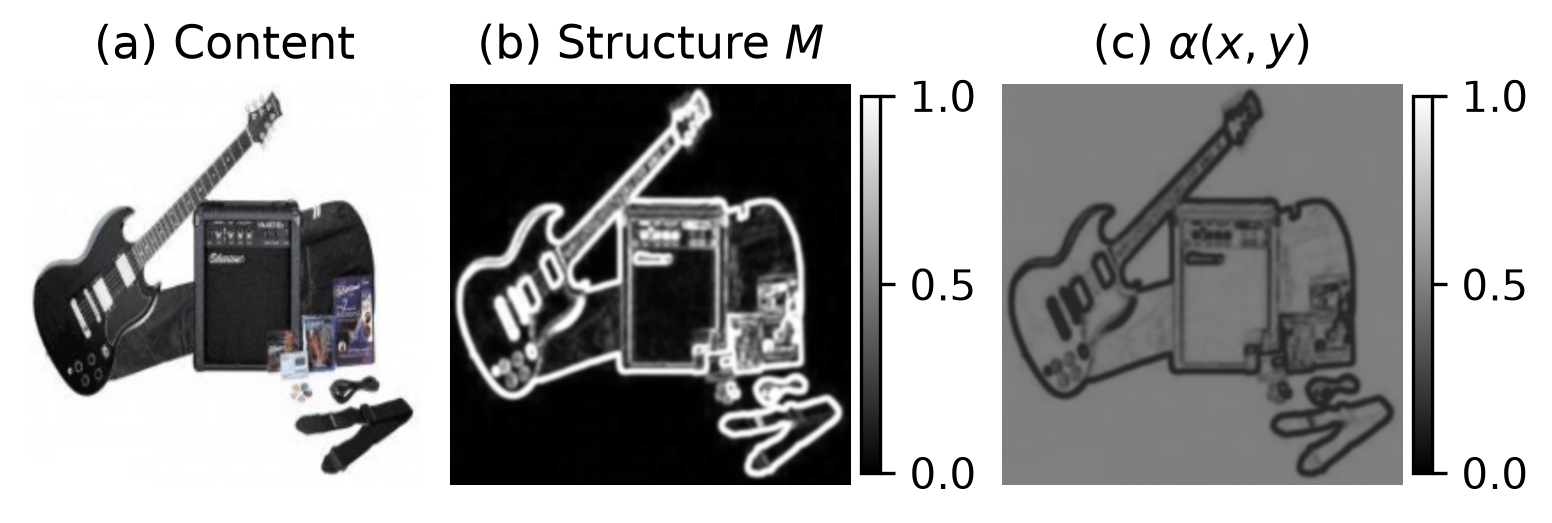
\includegraphics[width=\columnwidth]{m3_structure_alpha.png}
\caption{Actual Photo Training example: content image, soft structure response
$M$, and spatial strength $\alpha(x,y)$ for $\alpha_0=0.5$, $\beta=0.7$.
Both map color scales are fixed to $[0,1]$. Brighter $M$ produces lower local
style strength. The map also responds to background contours.}
\label{fig:m3_maps}
\end{figure}

\begin{figure*}[t]
\centering
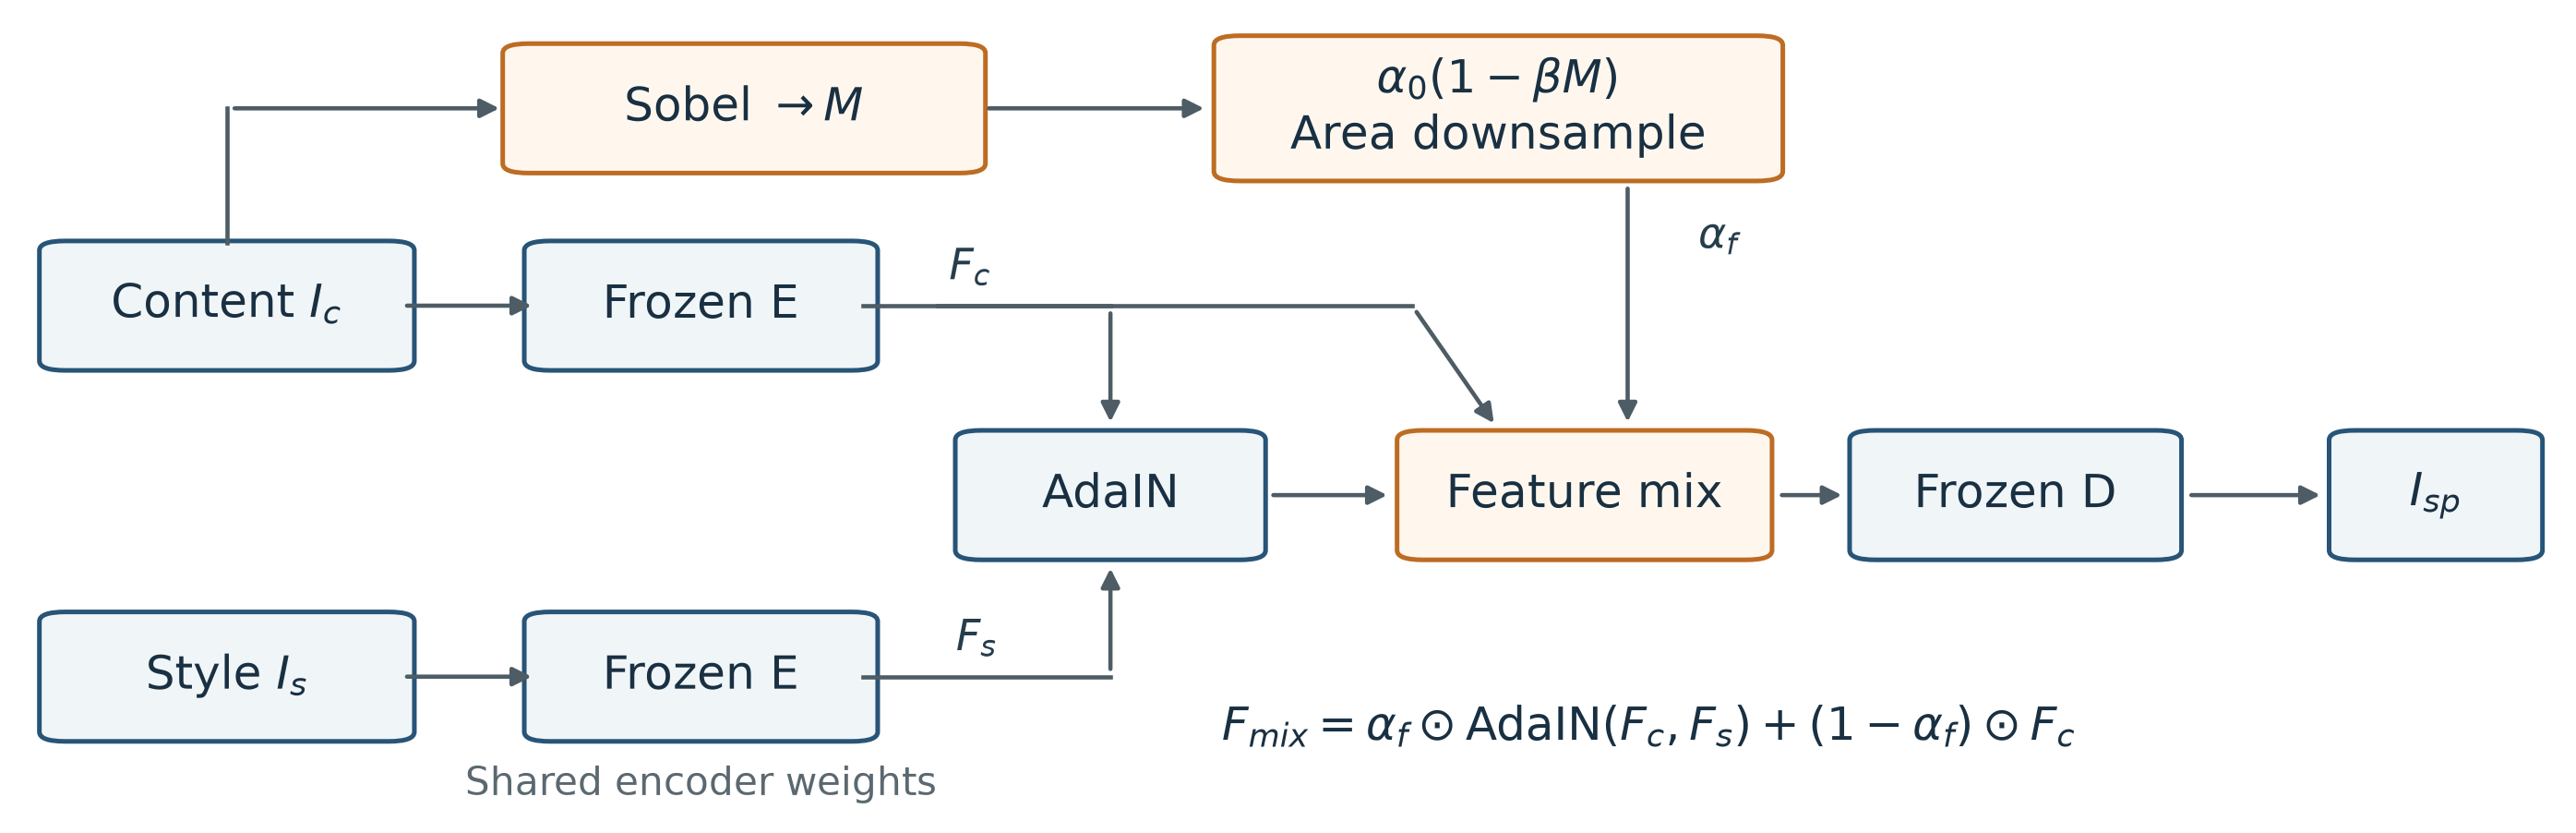
\includegraphics[width=0.96\textwidth]{m3_pipeline.png}
\caption{Structure-guided feature mixing. The structure branch uses the content
image only; the style reference changes feature statistics. Encoder and decoder
weights remain frozen.}
\label{fig:m3_pipeline}
\end{figure*}

\textit{Offline delivery and limitations.} The initial full set uses
$\alpha_0=0.5$, $\beta=0.7$ and contains one output for each of the 1,349 source
training images. The latter parameter is an initial setting, not a selected optimum.
Images are written to \texttt{data/aug\_sp/}; a manifest records the output path,
label, original, style, $\alpha_0$, and $\beta$. Geometry, frozen weights,
content--style pairing, and JPEG quality 95 are held fixed relative to the matched
AdaIN reference. Output dimensions follow the same decoder behavior in both
methods. The map is an edge-based proxy and cannot guarantee object preservation
after decoding. Since the rule also lowers mean style strength, a uniform control
with matched mean strength is needed to isolate the effect of spatial placement.

\setcounter{section}{3}
\section{Progress / Current Status}
\setcounter{subsection}{2}
% Exactly three current-status bullets for the progress report.
\subsection{Structure-Preserving Method Progress}
\label{sec:m3_current_status}
\begin{itemize}
\item \textit{Implementation completed.} We implemented the soft Sobel structure
map, adaptive strength $\alpha_0(1-\beta M)$, feature-level AdaIN mixing, batch
generation, diagnostic panels, and parameter sweeps on top of the pinned member-2
interface. Twelve automated tests passed, including constant-image handling,
parameter boundaries, recovery from corrupt outputs, manifest compatibility,
and equivalence between $\beta=0$ and ordinary AdaIN.

\item \textit{Full training augmentation delivered locally.} The generator
produced 1,349 real Photo Training augmentations in \texttt{data/aug\_sp/} at
$\alpha_0=0.5$, $\beta=0.7$. All outputs were decoded and checked for labels,
frozen pairings, input/output hashes, and manifest consistency. Two-column and
six-column manifests are available; the latter is directly readable by member 4.
Seven class examples with structure and strength maps are included in the handoff.

\item \textit{Analysis prepared; classification evaluation pending.} The full
set has EdgeScore $0.3436\pm0.0628$ over 1,349 images, where the spread is across
images, not classifier seeds. A five-value $\beta$ pilot was completed on seven
dog images; it demonstrates the generation workflow and is not a full ablation.
LPIPS and augmented-group classification results remain pending. Code, figures,
manifests, audit records, and the ablation plan are ready for integration.
\end{itemize}

\setcounter{section}{4}
\section{Next Steps and Plan for Completion}
\setcounter{subsection}{2}
% Member 3 contribution to Section 5.3; merge with member 4's training plan.
\subsection{Ablation and Analysis Plan}
\label{sec:m3_ablation_plan}

\textit{Protection-strength ablation.} We will hold $\alpha_0=0.5$ fixed and
generate $\beta\in\{0,0.3,0.5,0.7,1\}$ variants for the same 1,349 Photo Training
images. The style pool, content--style pairing, map settings, input sizes,
augmentation count, and image encoding will remain unchanged. The $\beta=0$
case is ordinary AdaIN and serves as the implementation and experimental control.
Member 3 provides images and manifests; member 4 performs classifier training and
evaluation under the shared protocol. The existing seven-image, dog-only pilot
checks execution and does not select an optimal $\beta$.

\textit{Structure and appearance analysis.} For every variant, we will compute
the fixed-threshold Canny EdgeScore and LPIPS, using the same preprocessing as
Section~3.6. We will report means, image-level standard deviations, valid counts,
and per-image differences relative to $\beta=0$. Empty-edge cases will remain
undefined and their number will be disclosed. LPIPS is planned and has not yet
been computed. Qualitative panels will use fixed $[0,1]$ map scales and matched
content/style pairs across classes. We will inspect thin structures, textured
backgrounds, and failures where the map protects irrelevant edges.

\textit{Reduced-strength confound.} Increasing $\beta$ decreases average style
strength as well as adding spatial modulation. A recommended additional control
is uniform AdaIN with per-image strength
\begin{equation}
\bar\alpha_i=\frac{1}{H_fW_f}\sum_{u,v}\alpha_{f,i}(u,v).
\label{eq:m3_mean_match}
\end{equation}
It uses the same content/style pair and decoder. This control is a proposed
extension, not an output already produced by the current batch CLI. Comparing
it with the spatial map would help separate the effect of where protection is
applied from the effect of weaker stylization alone.

\textit{Classifier analysis and parameter discipline.} Member 4 will use the
shared ResNet-18, batch size 64, 660 optimizer steps, and final-checkpoint policy.
A one-seed sweep can provide an exploratory budget; the primary comparison and
any configurations used for a replicated claim will use seeds $\{0,1,2\}$.
We will report Photo accuracy separately from the unweighted average of Art,
Cartoon, and Sketch accuracies, with per-domain and relevant per-class results.
Target-domain test data will not choose $\alpha$, $\beta$, map settings, or
checkpoints. Any selection rule will be fixed in advance or use source validation
only; the initial $\beta=0.7$ is retained as a predeclared setting. Higher EdgeScore
or lower LPIPS will be treated as image analysis rather than proof of a classifier
gain. A later alpha sweep may use $\{0.25,0.5,0.75,1\}$ with its beta held fixed
to avoid confounding both factors in the main beta comparison.

\bibliographystyle{plain}
\bibliography{references}
\clearpage
\onecolumn
\section*{Supplementary Figure Material}
\begin{center}
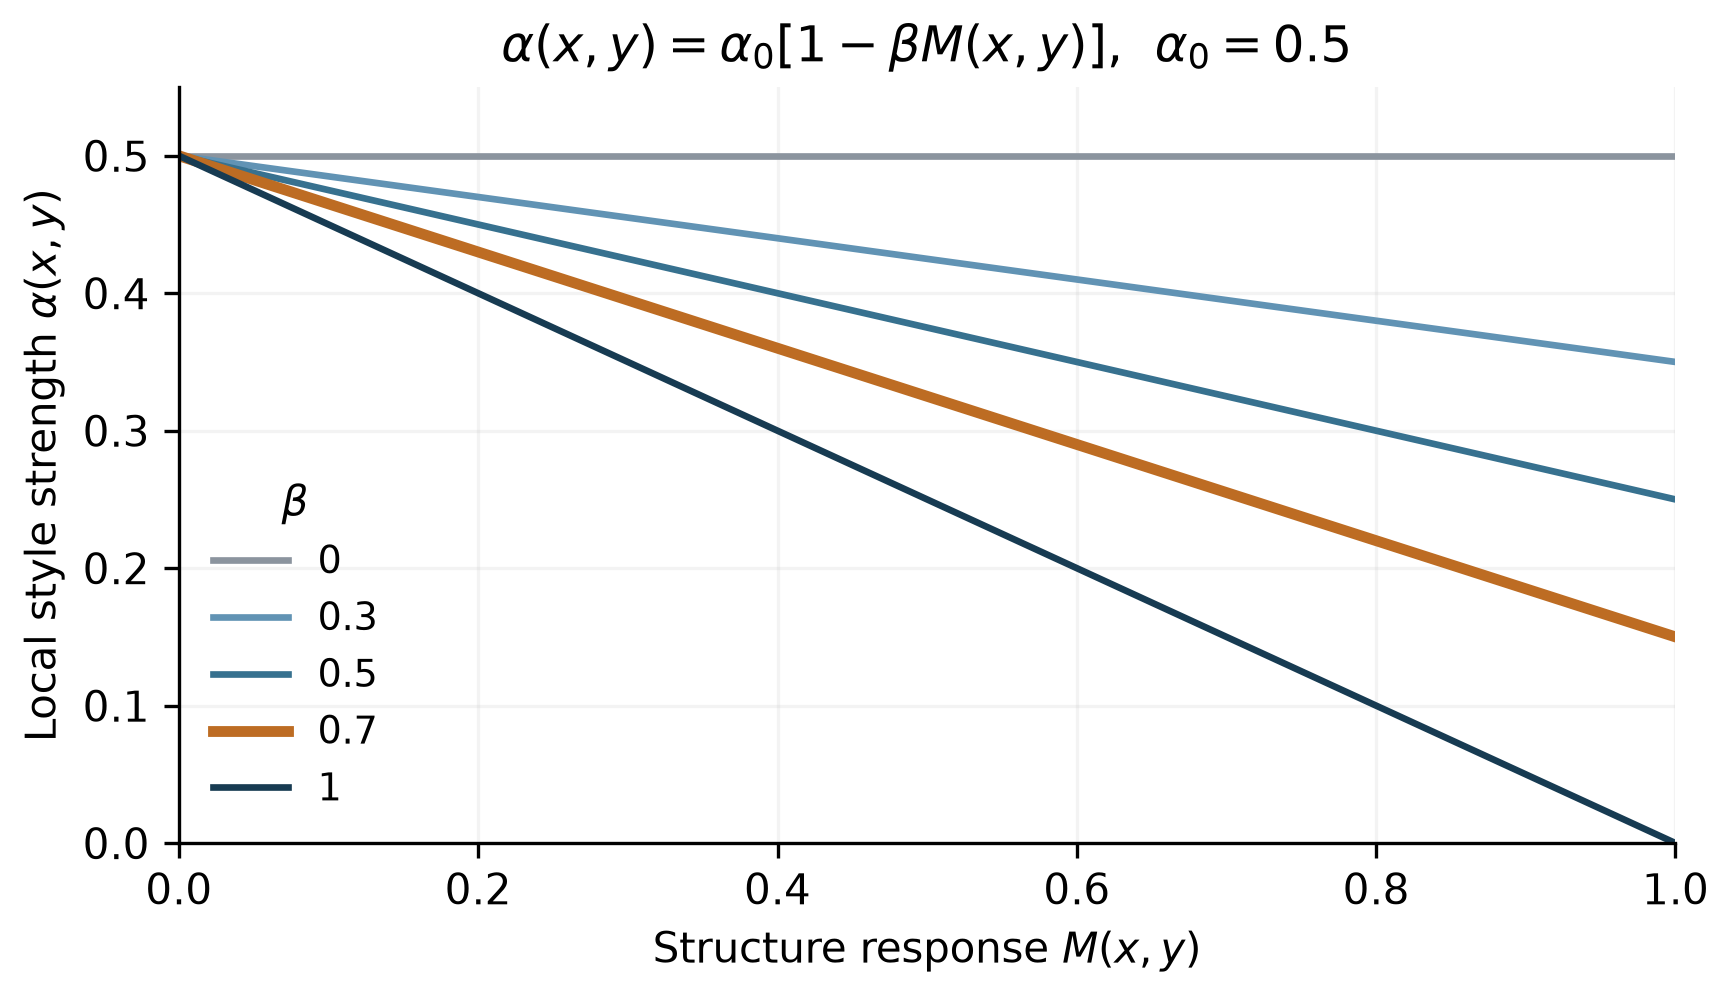
\includegraphics[width=0.64\textwidth]{m3_alpha_rule.png}
\end{center}
\noindent\textbf{Analytical strength rule.} Fixed base strength is 0.5. Larger
$\beta$ lowers local strength where the structure response is stronger.
\begin{center}
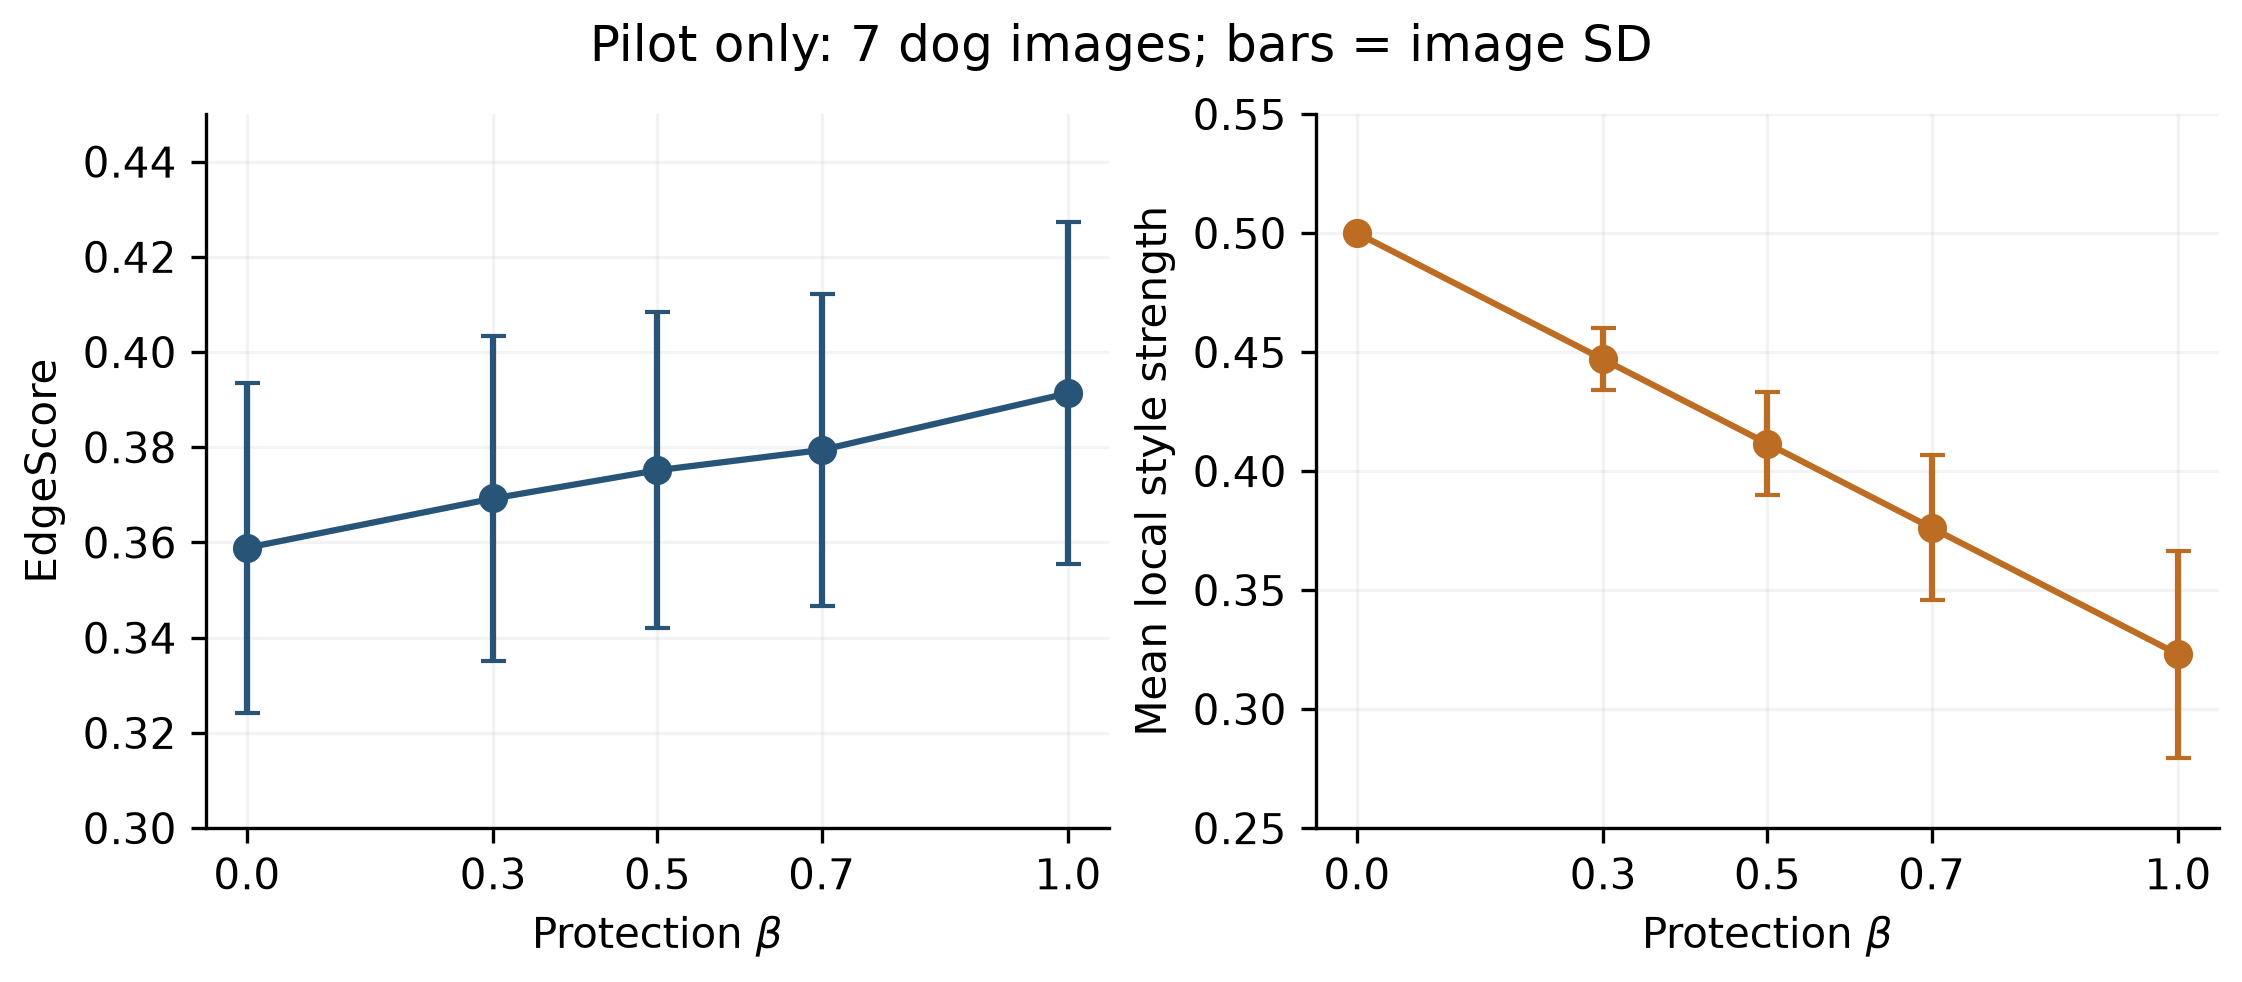
\includegraphics[width=0.88\textwidth]{m3_beta_pilot.png}
\end{center}
\noindent\textbf{Pilot only.} Seven dog images; error bars are image-level standard
deviations. This pilot does not establish an optimal parameter or a classification gain.
\begin{center}
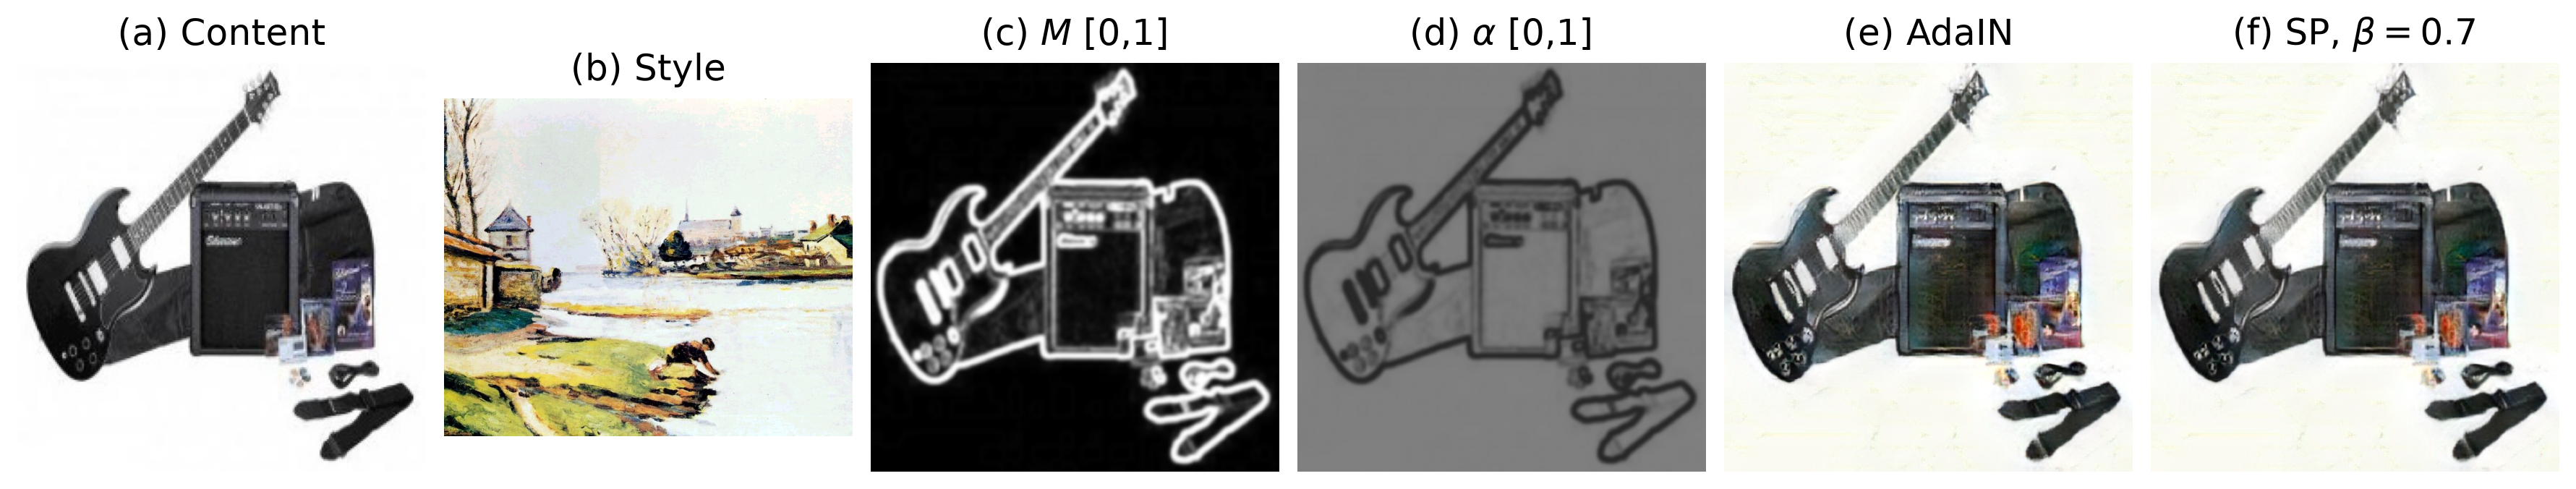
\includegraphics[width=\textwidth]{m3_guitar_comparison.png}
\end{center}
\noindent\textbf{Qualitative example.} Content, style, structure response, spatial
alpha, matched ordinary AdaIN, and structure-preserving output. This is not a classifier result.
\end{document}
